% Faithful native paths from source/普通高考/2007/2007新课标文(海南,宁夏).pdf, page 1.
% Original outlines, connected rock fissures, solid/dashed edges and shaded regions retained.
% Labels retain their original objects; no arbitrary geometric substitute or raster wrapper.
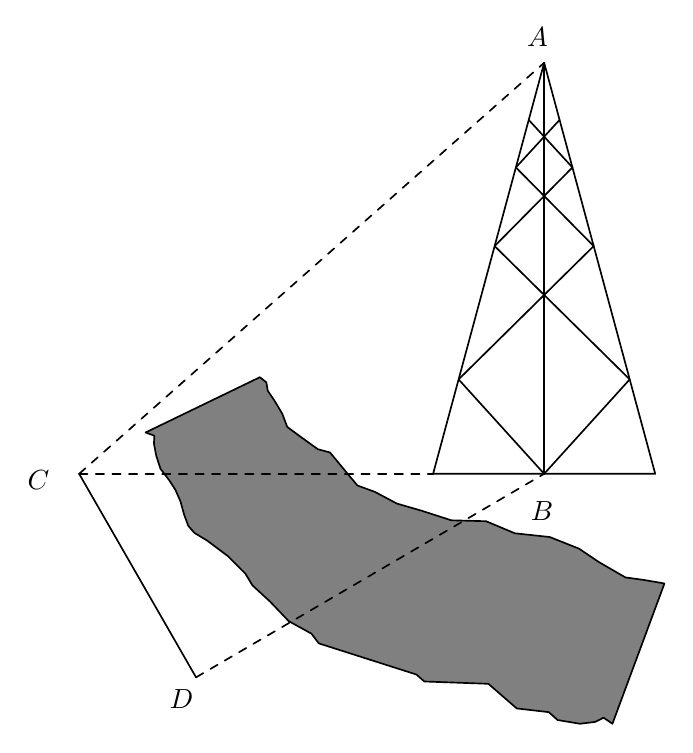
\begin{tikzpicture}[x=1cm,y=1cm,font=\normalsize,line join=round,line cap=round]
\path[draw=black,line width=0.6pt,fill=black!50] (2.04056,4.16785) -- (2.15266,4.12656) -- (2.14675,4.02628) -- (2.17622,3.87285) -- (2.22937,3.70771) -- (2.34141,3.56018) -- (2.41813,3.44218) -- (2.48304,3.29471) -- (2.53022,3.12361) -- (2.58332,2.98205) -- (2.66004,2.89352) -- (2.82517,2.79323) -- (3.08480,2.59857) -- (3.30899,2.37438) -- (3.39746,2.22685) -- (3.62165,2.02038) -- (3.85765,1.77262) -- (4.14674,1.61328) -- (4.24113,1.48943) -- (5.48002,1.09415) -- (5.58036,1.00567) -- (6.39450,0.97615) -- (6.75441,0.66348) -- (7.16145,0.61624) -- (7.27355,0.51595) -- (7.55674,0.46876) -- (7.75140,0.49239) -- (7.85759,0.54548) -- (7.96974,0.46876) -- (8.63044,2.25047) -- (8.35316,2.29766) -- (8.13487,2.32719) -- (7.79864,2.52186) -- (7.54493,2.69295) -- (7.17326,2.84042) -- (6.73079,2.88767) -- (6.36497,3.04105) -- (5.92250,3.05280) -- (5.53908,3.17671) -- (5.23227,3.26524) -- (4.95498,3.41271) -- (4.73079,3.49528) -- (4.60705,3.64313) -- (4.38269,3.91419) -- (4.22931,3.95547) -- (4.10541,4.04394) -- (3.97565,4.13838) -- (3.83993,4.23866) -- (3.77503,4.40976) -- (3.67704,4.57314) -- (3.59218,4.69880) -- (3.57446,4.80504) -- (3.49184,4.86989) -- (2.04056,4.16785) ;
\path[draw=black,line width=0.6pt] (1.19701,3.64315) -- (2.68181,1.05818) ;
\path[draw=black,line width=0.6pt] (5.69206,3.64315) -- (8.51308,3.64315) -- (7.10260,8.86295) -- (5.69206,3.64315) ;
\path[draw=black,line width=0.6pt] (7.10258,3.64315) -- (7.10258,8.86295) ;
\path[draw=black,line width=0.6pt] (6.90667,8.13798) -- (7.46168,7.53409) ;
\path[draw=black,line width=0.6pt] (7.29849,8.13798) -- (6.74348,7.53409) -- (7.73156,6.53529) -- (6.01606,4.84216) -- (7.10256,3.64313) -- (8.18912,4.84216) -- (6.47357,6.53529) -- (7.46171,7.53409) ;
\path[draw=black,line width=0.6pt,dash pattern=on 3pt off 3pt] (1.19701,3.64315) -- (5.69208,3.64315) ;
\path[draw=black,line width=0.6pt,dash pattern=on 3pt off 3pt] (1.19701,3.64315) -- (7.10256,8.86295) ;
\path[draw=black,line width=0.6pt,dash pattern=on 3pt off 3pt] (2.68182,1.05817) -- (7.10258,3.64313) ;
\node[anchor=base west,inner sep=0pt,outer sep=0pt] at (6.93246,3.04855) {$B$};
\node[anchor=base west,inner sep=0pt,outer sep=0pt] at (6.88729,9.06899) {$A$};
\node[anchor=base west,inner sep=0pt,outer sep=0pt] at (0.54330,3.44695) {$C$};
\node[anchor=base west,inner sep=0pt,outer sep=0pt] at (2.34640,0.65693) {$D$};
\end{tikzpicture}
